\documentclass[border=1pt]{standalone}
\usepackage{tikz}

\begin{document}
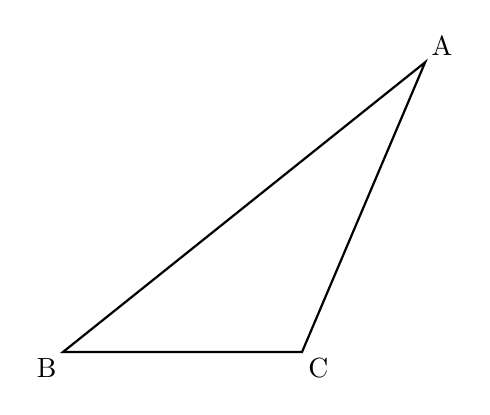
\begin{tikzpicture}
    \pgfmathsetmacro{\xa}{4.6}
    \pgfmathsetmacro{\xc}{\xa*0.66}
    \pgfmathsetmacro{\ya}{\xa*0.8}

    \coordinate (B) at (0,0);
    \coordinate (C) at (\xc,0);
    \coordinate (A) at (\xa,\ya);
    
    \draw [thick] (A)--(B)--(C)--cycle;
    \node[below left, outer sep=-1pt] at (B) {B};
    \node[below right, outer sep=-1pt] at (C) {C};
    \node[above right, outer sep=-1pt] at (A) {A};
\end{tikzpicture}
\end{document}

